
In order to choose the best working conditions for a group of people it is necessary to establish, whether climate of a particular place plays any part in determining an individual's productivity.

The first aspect of a climate that we are going to be examining is its temperature. A number of studies \CN{Taylor,2015} \CN{Muller,2012} have shown, that temperature does in fact have a considerable impact on human cognitive functions. One scientific paper in particular, however, has shown to be an invaluable source, when it comes to determining the extent of this impact. A NBER working paper from 2013 \CN{Chetty2013} has studied the correlation, between productivity and indoor temperature. This research presents us with several important observations. Firstly, the ideal temperature for mental work is around $22\degree C$. We can also use the data measured in this study in order to estimate the a function to determine the productivity of a person working in a given temperature.

\begin{figure}[ht]
	\centering
    	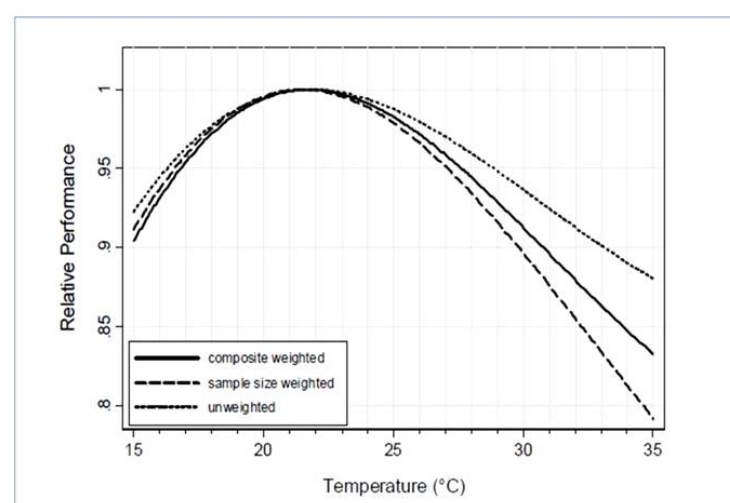
\includegraphics[width=0.4\textwidth]{graph_temp}
    \caption{Task performance vs. temperature \CN{Chetty2013}}
\end{figure}

Using the least-squares fit we arrived at an approximation of:

$$P\approx -1.06907 \cdot 10^{-7} \cdot t^{4}+0.00003 \cdot t^{3}-0.00344 \cdot t^{2}+0.11109 \cdot t-0.08269$$

\begin{figure}[ht]
	\centering
    	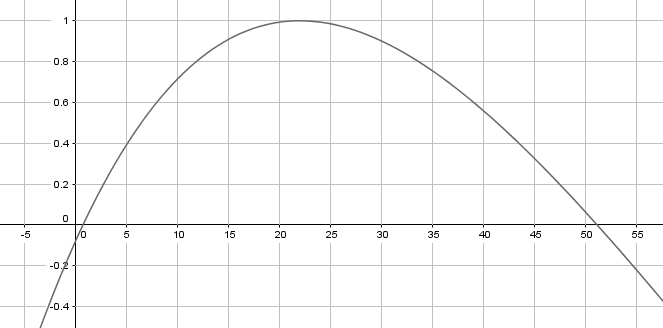
\includegraphics[width=0.4\textwidth]{graph4}
    \caption{Task performance vs. temperature, function fit}
\end{figure}

This approach does, however have its shortcomings. The first problem we have to consider, is that the original research only studied the effects of indoor temperature. In our case, indoor temperature is not so dependent on a particular city, since it can be easily controlled by heating or air conditioning. We can, however, predict, that outside temperature is going to have an effect on productivity, whether it be by decreasing comfort while traveling, or in case the outside temperature cannot be entirely differentiated from the indoor one, because of insufficient heating, insulation etc. We therefore decided to model the relationship between productivity and outside temperature based on the model for indoor temperature, since we can safely assume that both models behave similarly. To estimate an individual's productivity in this case, we will use the function mentioned above, using a parameter, that will determine the magnitude of performance impact.

$$P=\left( (-1.06907 \cdot 10^{-7} \cdot t^{4}+0.00003 \cdot t^{3}-0.00344 \cdot t^{2}+0.11109 \cdot t-0.08269)-1 \right)\cdot K_{T}+1$$

Where $K_{T}$ is the temperature effect parameter. For the purposes of this model, we estimate this value to be around:


